					%  tipo de documento
\documentclass[11pt]{amsart}

\usepackage[spanish,galician]{babel}
\usepackage[utf8]{inputenc}

					%  pinta dos folios
\usepackage[a4paper]{geometry}
\newgeometry{top=3cm,left=3cm,bottom=3cm}   
					%  símbolos matemáticos
\usepackage{amssymb,amsmath}
\usepackage{graphicx}
%\usepackage{epsfig} 	% for figures
%\usepackage{xcolor} 	% for color

%ligazóns
\usepackage{hyperref}	


%Loren ipsum
\usepackage{blindtext}

%------------------	
%  interlineado	
%------------------				
\renewcommand{\baselinestretch}{2}
\linespread{2}

%------------------	
%  título e autor	
%------------------		
\title{Configuración }		%vai aparecer na cabeceira das páxinas impares
\author{mesmamente} 	%vai aparecer na cabeceira das páxinas pares

\begin{document}
%----------------------------------------------------------------------------------------------------------------
% Logo i-rochiño
%----------------------------------------------------------------------------------------------------------------
\begin{figure}[ht]
	\raggedright
	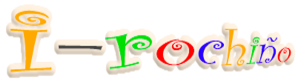
\includegraphics[width=4cm]{i-rocho.png}
\end{figure}

\maketitle %  velaquí vai o título e autor se procede
\thispagestyle{empty} % esta primeira páxina non leva número de páxina


%----------------------------------------------------------------------------------------------------------------
% Contido
%----------------------------------------------------------------------------------------------------------------
%\large
\section{ventilación}

\blindtext
\blindtext\blindtext\blindtext\blindtext\blindtext\blindtext






%------------------	
%  Páxina en branco sen número de páx
%------------------	
\clearpage\thispagestyle{empty}\null\newpage

%------------------	
%  Bibliografía	
%------------------	
\begin{thebibliography}{1}
\bibitem{washizu} Guia
\bibitem{paus} Pos escribui un libro de viaxes hai moooito tempo 
\end{thebibliography}


\end{document}  

















